\documentclass[12pt, a4paper]{article}
\usepackage[utf8]{inputenc}
\usepackage{listings}
\usepackage{courier}
\usepackage{fancyhdr}
\usepackage{color}
\usepackage{xcolor}
\usepackage{caption}
\usepackage{graphicx}
\usepackage{url}
\usepackage[titletoc]{appendix}
\usepackage{textcomp}
\usepackage{pdfpages}
\usepackage[colorlinks]{hyperref}
\hypersetup{urlcolor=blue}


\definecolor{light-gray}{gray}{0.95}

\lstset{
 upquote=true,
 showspaces=false,
 showtabs=false,
 frame=none,
 tabsize=2,
 breaklines=true,
 numbers=none,
 showstringspaces=false,
 breakatwhitespace=true,
 escapeinside={(*@}{@*)},
 keywordstyle=\bfseries,
 basicstyle=\footnotesize\ttfamily,
}

\newcommand{\code}[1]{{\footnotesize\texttt{#1}}}

\setlength\parindent{0pt} % Indentazione paragrafi
\setlength{\parskip}{1ex plus 0.5ex minus 0.2ex} % Spaziatura paragrafi


\title{
  
\includegraphics[width=0.8\textwidth]{img/logo.png}~ \\
  Inter-RAT handover (E-UTRAN to UTRAN) \\ \large Computer Networks module - LTE assignment
}
\author{Michele Zanotti}
\date{Spring term 2018}

\pagestyle{fancy}
\fancyhf{}
\lhead{Computer Networks}
\rhead{LTE assignment}
\rfoot{\thepage}


\begin{document}


\maketitle
\begin{figure}[htb]
	\centering
	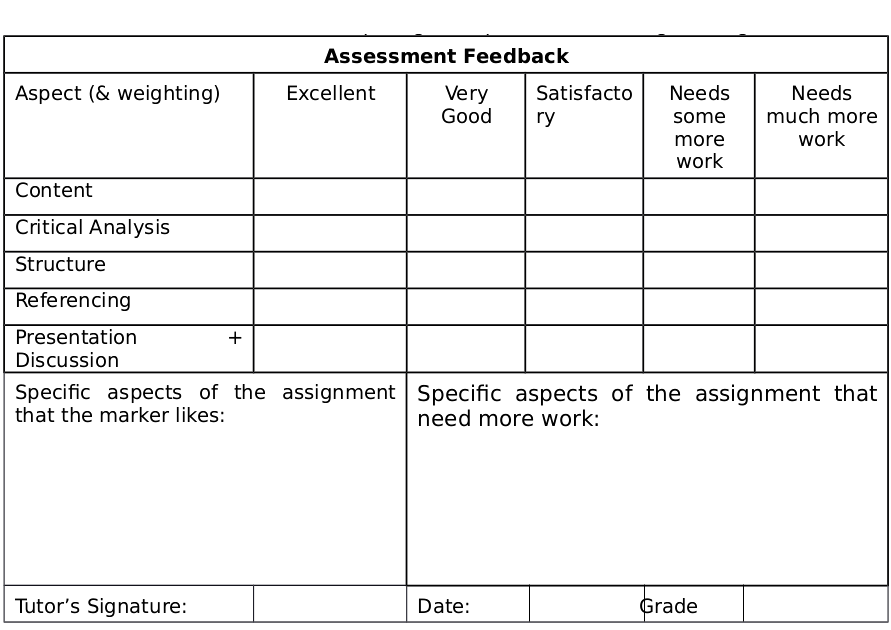
\includegraphics[width=1\linewidth]{img/valuation-table.png}
\end{figure}




\clearpage
\section*{List of Abbreviations}
\begin{tabular}{ p{4cm} l }
 3GPP & Third Generation Partnership Project \\
 CN & Core network \\
 CSG & Closed subscriber group (of a home eNodeB) \\
 E-UTRAN & Evolved UMTS terrestrial radio access network \\
 EPS & Evolved packet system \\
 GGSN & Gateway GPRS Support Node \\
 GTP & GPRS tunnelling protocol \\
 GTP-C & GPRS tunnelling protocol control part \\
 GTP-U & GPRS tunnelling protocol user part \\
 IMEI & International mobile equipment identity \\
 LTE & Long term evolution \\
 MME & Mobility management entity \\
 NSAPI & Network Service Access Point Identifier \\
 PDN & Packet data network \\
 PDU & Protocol data unit \\
 P-GW & Packet data network gateway \\
 RAB & Radio access bearer \\
 RNC & Radio network controller \\
 SDU & Service data unit \\
 SGSN & Serving GPRS Support Node \\
 S-GW & Serving gateway \\
 S-RNTI & Serving RNC Radio Network Temporary Identifier \\
 TEID & Tunnel endpoint identifier \\
 UE & User equipment \\
 UMTS & Universal Mobile Telecommunications System \\
 UTRAN & UMTS terrestrial radio access network \\


\end{tabular}

\clearpage
\section{Introduction}
The intra-RAT handover from E-UTRAN to UTRAN is composed of two phases, each of
which involves (as well as the UE) either nodes from the LTE network and nodes
from the UMTS netowork: the \emph{preparation phase} and the \emph{execution phase}.
In particular, the LTE elements involved in the procedure are:
\begin{itemize}
  \item eNodeB
  \item E-UTRAN network
  \item MME
  \item S-GW
  \item P-GW
\end{itemize}
while the UMTS elements are:
\begin{itemize}
  \item RNC
  \item SGSN
  \item GGSN
\end{itemize}

It is assumed that both the LTE and the UMTS networks belong to the same
operator. This means that the P-GW of the LTE network and the GGSN of the UMTS
network are the same physical device, therefore, since in this paper the focus
is on the LTE network, only the P-GW will be showed. Moreover, since the goal
of this paper is to show only the intra-RAT handover procedure, some non-central
aspects such as the relocation of the S-GW will not be considered and the related
messages and parameters will be left out.

It is important to point out that before, during and after the handover the UE
is in the state ``LTE\_ACTIVE'' and user data is uploaded/downloaded (otherwise
if the UE was in idle state it wouldn't be a handover but a simple cell reselection).
In particular, as shown in figure \ref{fig:pre-handover-links}, before the handover procedure both uplink
and downlink user data is transmitted through:
\begin{itemize}
	\item bearer(s) between UE and source eNodeB
	\item GTP tunnel(s) between	source eNodeB, S-GW and P-GW.
\end{itemize}


The figure \ref{fig:architecture-model} shows the elements involved in this
handover procedure, how they are connected to each other and through which
interfaces, figure \ref{fig:pre-handover-links} shows how data is transmitted
before the start of the procedure.

\begin{figure}[htb]
	\centering
	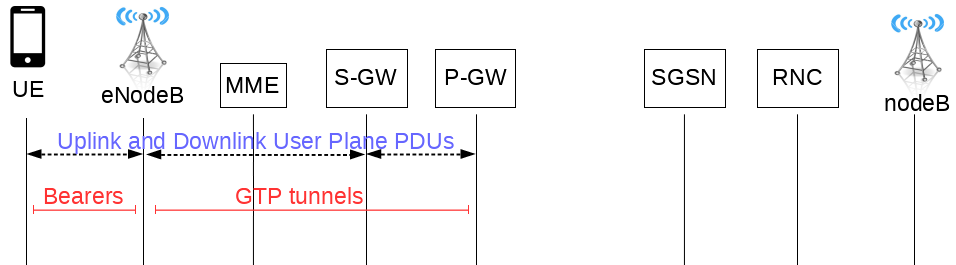
\includegraphics[width=1\linewidth]{img/pre-handhover-links.png}
	\caption{LTE and UMTS networks before the handover.}
  \label{fig:pre-handover-links}
\end{figure}

\begin{figure}[htb]
	\centering
	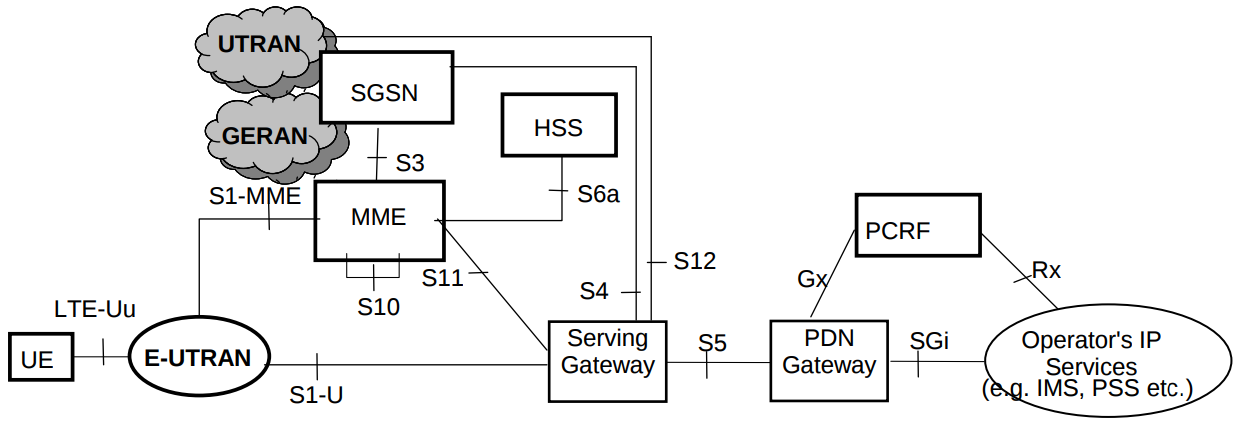
\includegraphics[width=1\linewidth]{img/architecture-reference.png}
  \caption{non-roaming architecture for 3GPP accesses.}
	\label{fig:architecture-model}
\end{figure}


\section{Preparation phase}
\begin{figure}[htb]
	\centering
	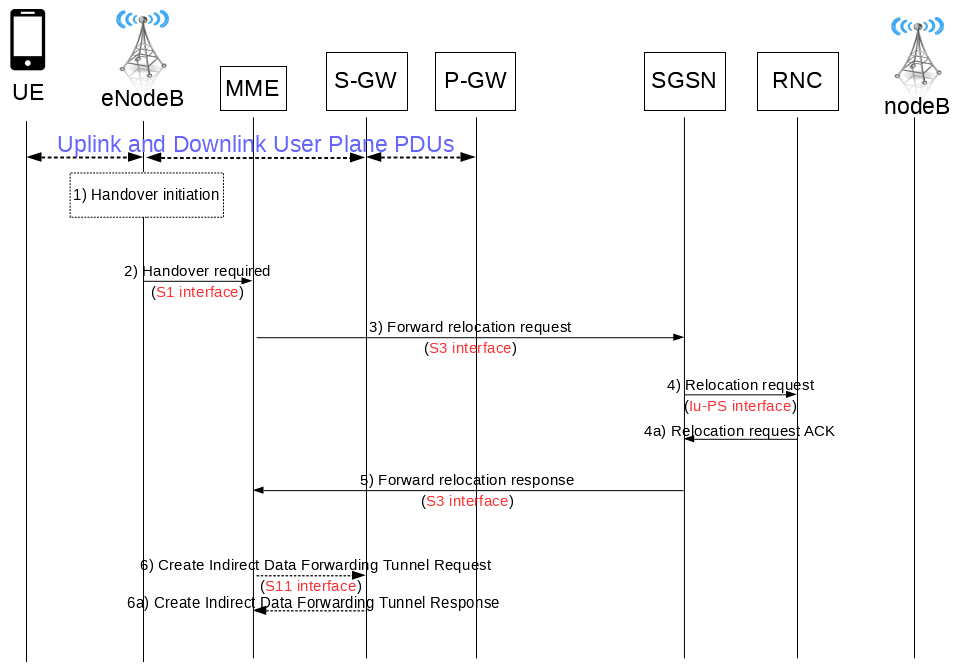
\includegraphics[width=1\linewidth]{img/preparation-phase.png}
	\label{fig:preparation-phase}
	\caption{the flow of the messages and the nodes involved in the
	handover preparation phase}
\end{figure}

\begin{itemize}
	\item [1)] The source eNodeB decides to initiate an Inter-RAT handover to the
	target access network
	\item [2)] The source eNodeB sends a \code{Handover Required} message to the
	source MME, requesting the CN to establish resources in the target RNC,
	target SGSN and the Serving GW. The message is sent through the S1 interface and
	it contains the following parameters:
	\begin{itemize}
		\item S1AP Cause: it specifies the reason of the message
		\item Target RNC Identifier: it identifies the target RNC
		\item CSG access mode: included only if the target cell is a hybrid cell
		\item CSG ID: included only if the target cell is a CSG\footnote{CSG = closed
		subscriber group of a home eNodeB} or hybrid cell, it	identifies the cell
	\end{itemize}
	\item [3)] The source MME determines from the ``Target RNC Identifier'' field that
	the type of handover is intra-RAT Handover to UTRAN Iu mode, then it
	initiates the Handover resource allocation procedure by sending a \code{Forward
	Relocation Request} message to the target SGSN. Some of the parameters included
	in this message are:
	\begin{itemize}
		\item user IMSI
		\item ISR Supported: it indicates if the source MME and the source S-GW are
		able to activate ISR\footnote{ISR = ``idle mode signalling reduction''. When
		this mode is active the network can simultaneously register the UE in a
		routing area that is served by an SGSN and in one or more tracking areas
		that are served by an MME.}
		\item PDN connections: it indicates the active PDN connections
		\item RAN cause: it's the S1AP cause received from the eNodeB
	\end{itemize}


http://www.etsi.org/deliver/etsi_ts/123400_123499/123401/14.07.00_60/ts_123401v140700p.pdf

\section{Execution phase}



\subsection*{Step 1}
The source MME completes the preparation phase by sending to the source eNodeB
the \emph{Handover command} message through the interface S1. The message
contains the following parameters:
\begin{itemize}
    \item Target to Source Transparent Container
    \item E-RABs to Release List
    \item Bearers Subject to Data Forwarding List: if ``Direct
    Forwarding'' applies it is the list of ``Address(es) and TEID(s) for user
    traffic data forwarding'' received from the target SGSN during step 7
    of the preparation phase, otherwise if ``Indirect Forwarding'' applies
    it contains the parameters received in step 8a from the S-GW
    \item E-RABs to Release List
\end{itemize}




\subsection*{Step 2}
The source eNodeB initiates data forwarding for bearers specified in the
``Bearers Subject to Data Forwarding List'' of the message received from the MME.

After that, the eNodeB sends the E-UTRAN command \emph{HO} to the UE for telling
it to handover to the target access network. This message includes a transparent
container which contains the radio parameters that the RNC has set-up during the
preparation phase.

After the reception of the HO command the UE has to associate its bearer IDs to
the respective RABs according to the relation with the NSAPIs\footnote{NSAPI =
Network Service Access Point Identifier, it is used to identify PDP contexts in
the SGSN. A PDP context is a data structure which contains subscriber's session
information such as its IMSI and its IP address} and has to suspend
the uplink transmission of user data.



\subsection*{Step 3}
Void




\subsection*{Step 4}
The UE executes the handover to the target UTRAN according to the prameters
contained in the message received in step 2. At this point it can resume the user
data transfer only for those NSAPIs which have been associated to a RAB, namely
the NSAPIs for which there are radio resources allocated in the target RNC.




\subsection*{Step 5}
After the RNC-ID and the S-RNTI\footnote{S-RNTI = Serving RNC Radio Network
Temporary Identifier, in UMTS the S-RNTI is the UE identifier which is allocated
by the RNC and it's unique within that RNC} are exchanged with the UE, the target
RNC sends the \emph{Relocation Complete} message to the target SGSN, indicating
therefore the completion of the relocation from the source E-UTRAN to the target
RNC. After receiving this message, the SGSN is ready for receiving data from
the target RNC. 

\section{Handover reject}
\begin{figure}[htb]
	\centering
	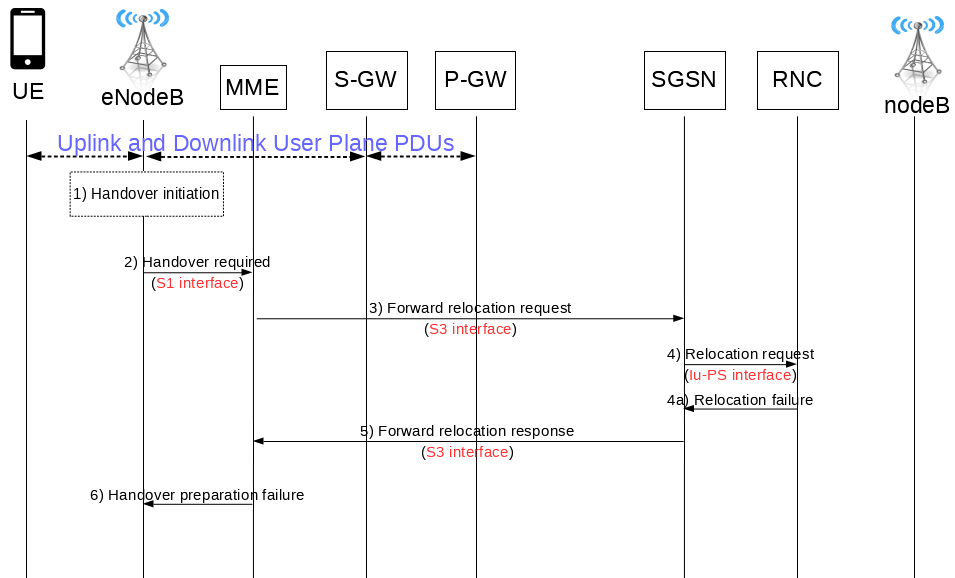
\includegraphics[width=1\linewidth]{img/handover-reject.png}
	\label{fig:preparation-phase}
\end{figure}

The Target RNC may reject the Handover if none of the RABs specified in the
Relocation Request message could be established. In this case no UE context is
established in the SGSN/RNC and no resources are allocated, the UE therefore
remains in the Source eNodeB/MME.



\subsection*{Step 1}
Step 1 to 4 are identical to the ones shown in the first chapter (Execution phase).



\subsection*{Step 4a}
The RNC fails to allocate any resources for any of the requested RABs, therefore
it sends to the SGSN a Relocation Failure message. When the SGSN receives the
Relocation Failure message it clears any reserved resources for this UE.



\subsection*{Step 5}
The SGSN sends the Forward Relocation Response message to the Source MME, specifying
the handover reject as parameter in the message (cause field).



\subsection*{Step 6}
When the MME receives the Forward Relocation Response message it sends a Handover
Preparation Failure message to the Source eNodeB.



\begin{thebibliography}{99}
\footnotesize

  \bibitem{direct-tunnelling}
  Cisco. (2017).
  \textit{P-GW Administration Guide, StarOS Release 20 - Direct Tunnel for 4G (LTE) Networks [Cisco ASR 5000 Series]}. [online]
  Available at: \url{https://www.cisco.com/c/en/us/td/docs/wireless/asr_5000/20/P-GW/b_20_PGW_Admin/b_20_PGW_Admin_chapter_011111.html}
  [Accessed 5 May 2018].

  \bibitem{routing-area-update}
  3GPP TS 23.401 (September 2011)
  \textit{General Packet Radio Service (GPRS) Enhancements for Evolved Universal
  Terrestrial Radio Access Network (E-UTRAN) Access},
  Release 10,
  sections 5.3.3.3, 5.3.3.6.

  \bibitem{channels}
  Poole, I. (n.d.).
  \textit{LTE Physical, Logical and Transport Channels :: Radio-Electronics.Com}. [online]
  Radio-electronics.com.
  Available at: \url{http://www.radio-electronics.com/info/cellulartelecomms/lte-long-term-evolution/physical-logical-transport-channels.php}
  [Accessed 16 May 2018].


\end{thebibliography}


\end{document}
